\documentclass[11pt,leqno]{article}
\usepackage[polish]{babel}
%\usepackage[OT4]{polski}
\usepackage[utf8]{inputenc}
\usepackage[T1]{fontenc}
\frenchspacing
%\usepackage{indentfirst}
\usepackage{listings}
\usepackage{framed}
\usepackage[textwidth=16cm,textheight=24cm]{geometry}
\usepackage{graphicx}
\usepackage{hyperref}
%\graphicspath{{img\\}}

\usepackage{subfig}
\setlength\fboxsep{0pt}
\setlength\fboxrule{0.5pt}

\newcommand{\myimage}[3]{
  \begin{figure}[h!]
    \centering
      \includegraphics[scale=#1]{#2}
  \caption{#3}
  \end{figure}
}

\usepackage{float}
\floatstyle{boxed} 
\usepackage{wrapfig}

\usepackage{fancyhdr}
\pagestyle{fancy}
%\fancyhf{}
\cfoot{\thepage}
\lhead{\nouppercase{\leftmark}}
\rhead{\nouppercase{\rightmark}}


\title{\normalsize \textbf{Studencka Pracownia Licencjackiego Projektu Programistycznego} \\
       \textbf{II UWR 2010/2011} \\ 
       \ \\
       \vspace{15em}
       \Large Wojciech Jedynak \\
       \normalsize \ \\
       \Huge GoStat \\
       \tiny \ \\
       \LARGE \textbf{Program do wykonywania obliczeń} \\
              \textbf{statystycznych związanych z grą go} \\ 
       \ \\
       \Large Motywacja dla projektu \\
       \vspace{15em}
       }

\date{Wrocław, \today}

\begin{document}

\maketitle 
\thispagestyle{empty}

\newpage

\tableofcontents

\newpage


\section{Wprowadzenie do gry go}

\subsection{Charakterystyka i zasady}

Go jest strategiczną grą planszową pochodzenia chińskiego. Należy zarówno do jednych z nastarszych gier znanych 
ludzkości (niektórzy oceniają jej historię na około 4 tysiące lat), jak i do najtrudniejszych i najbardziej złożonych.
Liczba możliwych gier jest szacowana na nawet $ 10^{750} $, a średnio w każdej sytuacji gracz ma do wyboru około 200 możliwości.
% Bardzo trudno napisać program komputerowy, który grałby dobrze w go. 

Go jest grą dla dwóch graczy. Rozgrywka toczy się na kwadratowej planszy przeciętej 19 liniami poziomymi i 19 liniami pionowymi 
tworzącymi 361 przecięć. Aby ułatwić naukę gry  początkującym, używa się również mniejszych plansz, 
o rozmiarach 9x9 oraz 13x13 (por. ilustracje poniżej).

Na samym początku rozgrywki plansza jest pusta, następnie gracze naprzemiennie kładą na wolnych przecięciach swoje pionki, 
zwane tutaj kamieniami. Gracz, który rozpoczyna partię używa kamieni czarnych, jego przeciwnik ma kamienie białe.

Pełne wprowadzenie do gry znajdziemy w witrynie go.art.pl \cite{rules}.

\begin{figure}[h!]
  \centering
  \subfloat[Tradycyjny japoński zestaw do gry w Go: kamienie (często wykonywane z muszli), plansza i pojemniki na kamienie.]
   {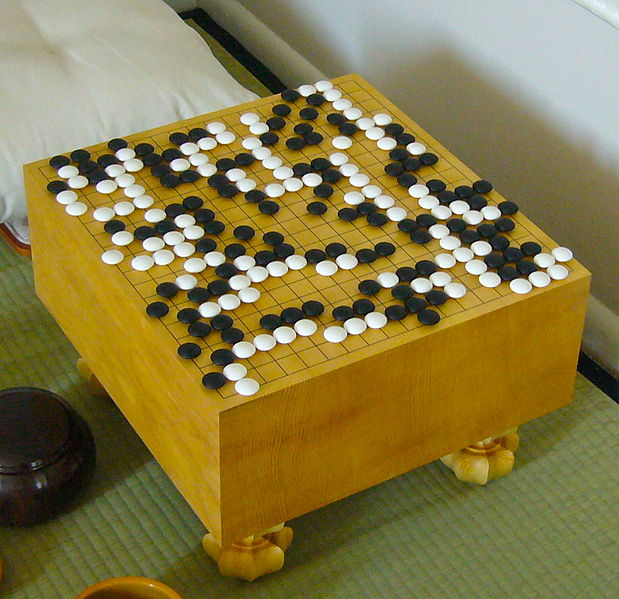
\includegraphics[width=0.4\textwidth]{619px-FloorGoban.JPG}}
  \hspace{0.5cm}                
  \subfloat[Plansza o oficjalnych rozmiarach (19 x 19)]{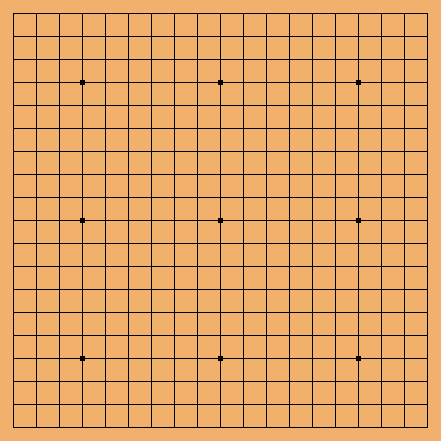
\includegraphics[width=0.4\textwidth]{19.png}}
  %\caption{Pictures of animals}
  
  \subfloat[Plansza pośrednia między 9x9 a 19x19: rozmiar 13x13]
   {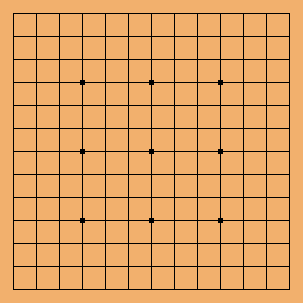
\includegraphics[width=0.4\textwidth]{13.png}}
  \hspace{0.5cm}                
  \subfloat[Najmniejsza plansza używana w praktyce (9x9)]{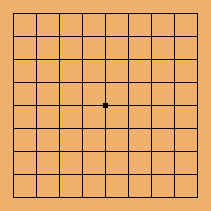
\includegraphics[width=0.4\textwidth]{9.png}}
  %\caption{Pictures of animals}
\end{figure}

\subsection{Popularność gry }

Gra cieszy się ogromną popularnością w Azji wschodniej, gdzie grają w nią setki milionów osób. Na zachodzie go jest mniej znane, 
jednak w bardzo wielu krajach istnieją stowarzyszenia, które zrzeszają miłośników gry. 

W Polsce od 1983 roku istnieje Polskie Stowarzyszenie Go \cite{psg}, 
rozgrywana jest Liga Mistrzostw Polski, a także Mistrzostwa Polski Kobiet, Par i Juniorów. 

Istnieje kilkanaście klubów, w których regularnie odbywają się spotkania goistyczne 
-- we Wrocławiu funkcjonują dwa kluby: jeden na Wydziale Fizyki UWr \cite{gokurabu}, drugi na Politechnice \cite{sente}.

 Na liście rankingowej przeważnie znajduje się od około 300 do 400 osób z całego kraju \cite{ranking}.

Aktualnym mistrzem Polski jest Leszek Sołdan, zaś na rozgrywanych rokrocznie w Japonii Mistrzostwach Świata Amatorów 
reprezentował Polskę w 2011 roku Kamil Chwedyna (aktualny wicemistrz Polski) \cite{kamil1}. 
Kamil zajął rewelacyjne 13 miejsce \cite{kamil2} i otrzymał nagrodę specjalną za 
``swobodę i lekkość stylu'' od głównego sędziego zawodów, którym był sam Masaki Takemiya. 
Takemiya to legendarny japoński gracz zawodowy; odnosił w latach 1975-1990 ogromne sukcesy, a jego styl
gry był tak niekonwencjonalny, że był określany często ``Kosmicznym go''.

\subsection{Organizacje graczy zawodowych}
W Japonii, Chinach, Korei Południowej i na Tajwanie istnieją organizacje graczy zawodowych, którzy stanowią światową czołówkę konkurującą w 
prestiżowych turniejach o wysokie nagrody pieniężne. Ich poczynania śledzą pasjonaci go z całego świata. 

Wielu zawodowców zamiast na rywalizacji koncentruje się na nauczaniu i odwiedza turnieje na całym świecie, gdzie analizują 
partie amatorów, rozgrywają gry szkoleniowe i prowadzą wykłady. Liczna grupa wydaje książki z zadaniami treningowymi, 
poradniki strategiczne oraz leksykony zagrań o zaskakującej skuteczności. 
Tylko niewielka cześć wydawanych książek jest tłumaczona na język angielski, ale kilka wybitnych
 pozycji jest dostępnych jedynie w tym języku, gdyż opracowali je... zachodni amatorzy!

Co trzeba zrobić, by zostać zawodowcem? Przede wszystkim zacząć naukę gry w bardzo młodym wieku (około 5-8 lat), 
bardzo dużo ćwiczyć (najlepiej pod okiem nauczyciela-zawodowca) i odnieść sukces w organizowanym raz do roku egzaminie. 
To ostatnie jest wyczynem ekstremalnie trudnym. By podejść do tego egzaminu należy przejść przez kwalifikacje, następnie 
rozegrać grę z każdym z około 30 innych kandydatów i na koniec uplasować się w najlepszej trójce. 
Tak, tylko trzy osoby rocznie zasilają grono zawodowców...

Czy tylko Azjaci mogą uzyskać licencje zawodową? Niekoniecznie, choć wyjątki są bardzo nieliczne \cite{gopros}. Do tej pory udało
to się między innymi Rosjanom (Alexandre Dinerchtein, Svetlana Shikshina), Rumunowi (Catalin Taranu) i Amerykanom 
(Michael Redmond, James Kerwin).

\subsubsection{Polskie akcenty}

Próbował tego także czternastokrotny mistrz Polski Leszek Sołdan. Mimo że spędził wiele lat w Japonii 
trenując z elitą japońskich kandydatów na zawodowców (jap. insei), nie udało mu się zdać egzaminu. Być może sztuka 
ta uda się w przyszłości młodemu Mateuszowi Surmie. Jest on aktualnym mistrzem Europy do lat 16 (po raz drugi z rzędu) i plasuje się 
obecnie na drugiej pozycji w polskiej klasyfikacji turniejowej (tuż za Sołdanem) \cite{ranking}.

\subsection{Dalsze informacje}

Więcej informacji o go można znaleźć na stronie \url{http://go.art.pl}.

\section{Analiza statystyczna otwarć}

\subsection{Wprowadzenie}

Idea projektu GoStat powstała, gdy mój dobry kolega i wieloletni popularyzator go we Wrocławiu, Łukasz Fajfrowski opowiedział mi, że znalazł w sieci kolekcję 
kilkuset zapisów partii granych przez zawodowców na planszy 9x9. Probówał przygotować opracowanie najczęstszych oraz
najskuteczniejszych zagrań w początkowej fazie gry. Posiadanie (i przeanalizowanie) takiej bazy wiedzy pozwoliłoby na:

\begin{enumerate}
\item Podniesienie własnego poziomu gry poprzez wykorzystanie wiedzy i doświadczenia graczy zawodowych
\item Odkrycie, czy pewne zagrania są znacznie lepsze od innych, czy jest to jedynie kwestia indywidualnych preferencji
\end{enumerate}

Zestawienie było cenne tym bardziej, że w każdej partii wyjściowe ustawienie jest identyczne i gra jest w pełni deterministyczna,
W szczególności moglibyśmy choć trochę przybliżyć się do odpowiedzi na jedno z kluczowych pytań: czy w go czarny
 (czyli pierwszy gracz) ma strategię wygrywającą? Jeśli tak, to które ruchy dają pewną wygraną?

\subsection{Waga problemu}

Zagadnienie \emph{rozwiązania gry} fascynuje badaczy sztucznej inteligencji od lat,
 a próby napisania programu, który grałby dobrze w szachy podjęli nawet Turing i Shannon \cite{ai}.

Od 2007 roku znamy częściową  odpowiedź dla gry w warcaby \cite{checkers}. Trudno ocenić kiedy uda (czy) się ludzkości wyznaczyć odpowiedź dla gry w szachy. 

W przypadku go sytuacja wygląda tak, że przeanalizowano w pełni grę na planszy 4x4, 
zaś dla planszy 5x5 wykazano przy pomocy analizy komputerowej, że czarny zaczynając od zagrania w środek wygrywa \cite{gofive}. 

\subsection{Przyszłość}

Możemy oceniać, że przy nieustającym rozwoju sprzętu i postępach w pracy nad  algorytmami przeszukującymi drzewo
gry uda się w przyszłości uzyskać analogiczne wyniki dla planszy 9x9. Osiągnięto niesamowity progres w dziedzinie 
programów grających w go na planszy 9x9. W czerwcu 2011 roku mecz rozgrywany
między programem MyGoFriend a koreańskim zawodowcem Kim Young Sam zakończył się remisem 2:2 \cite{promatch}.

Należy jednak zwrócić uwagę, że z praktycznego punktu widzenia, plansza 9x9 jest tylko narzędziem treningowym w 
porównaniu z czterokrotnie większą (pod względem liczby przecięć), oficjalną planszą 19x19. Różnice w grze na obu planszach
 nie są jedynie kosmetyczne i ilościowe. Strategia gry na dużej planszy jest niemal zupełnie inna niż na planszy małej. \\
Przykładowo:
\begin{itemize}
\item Rozpoczęcie w środek na planszy małej to ruch, który ma wpływ na całą planszę. Analogiczne zagranie na planszy 19x19 nie ma takiego 
efektu, gdyż środek jest bardzo odległy od rogów, gdzie najłatwiej rozpocząć budowanie pozycji. Dla dużej planszy zagranie takie jest
 uważane za strategię na specjalne okazje.
\item Na dużej planszy najskuteczniejszym planem jest niekiedy poświęcenie dużej liczby kamieni, aby uzyskać przewagę w innym miejscu.
 Na mniejszych planszach manewr taki często kończy się przegraną, gdyż strata jest zbyt duża.
\end{itemize}

Biorąc dodatkowo pod uwagę, że znacznie trudniej jest ocenić jakość ruchu na planszy 19x19, jesteśmy w stanie zrozumieć, dlaczego 
nie ma do tej pory programów, które mogłyby się mierzyć z zawodowcami na dużej planszy, mimo sukcesów na planszy małej.

\section{Problemy z ręczną obróbką kolekcji gier}

Podczas ręcznego tworzenia swojego opracowania, Łukasz dopisywał kolejne warianty do jednego pliku SGF, który miał 
zawierać kilkanaście ruchów z każdej partii z dostępnego archiwum, i aktualizował na bieżąco dane statystyczne. Było to bardzo 
czasochłonne, żmudne i wymagało dużej koncentracji. Jednym z powodów tego był fakt, iż należało w pamięci dokonywać \emph{normalizacji}
 ruchów, aby wziąć pod uwagę symetrie. 

\begin{wrapfigure}{l}{0.3\textwidth}
  \vspace{-20pt}
  \begin{center}
    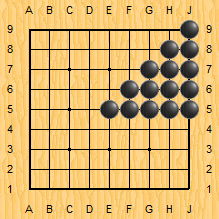
\includegraphics[width=0.28\textwidth]{symetria.png}
  \end{center}
  \vspace{-20pt}
  \caption{15 możliwych sposobów na rozpoczęcie gry, z dokładnością do symetrii \\i obrotów}
  \vspace{-10pt}
\end{wrapfigure}

Na planszy 9x9 mamy do dyspozycji 81 wolnych przecięć, ale z matematycznego punktu widzenia, zagrania w dowolny narożnik 
(A9, J9, A1, J1) są równoważne z dokładnością do obrotu lub symetrii. Jedynie ruch w sam środek jest pod tym względem unikatowy. 
Aby statystyka była poprawna, dwa symetryczne zagrania należy liczyć jako dwa wystąpienia tego samego ruchu! \\ 
Najmniej podatnym  na błędy rozwiązaniem wydaje się wybranie pewnego zbioru ruchów, które są parami różne także po uwzględnieniu przekształceń 
geometrycznych. Przykładowy taki zbiór oznaczono na ilustracji obok. Jak widać, ma on 15 elementów. Normalizacja ruchu polega
 więc na znalezieniu równoważnego ruchu, który należy do tych 15 wyróżnionych. Niedogodność, która się z tym wiąże polega na 
tym, że jeśli znormalizujemy pierwszy ruch danej partii, musimy w ten sam sposób przekształcić wszystkie następne ruchy z tej samej gry. 
Przykładowo, jeśli na czarnego F4 biały odpowiedział A6, to nie wystarczy jedynie przekształcić
F4 na F6 - musimy także zmienić A6 na A4.

Widzimy, że cały proces jest nieco za skomplikowany, a cała operacja zbyt żmudna, by wykonywać ją ręcznie dla więcej niż 
kilkunastu gier (przeciętna gra na planszy 9x9 trwa około 50 ruchów), a interesować nas mogą także kolekcje składające się
z dziesiątek tysięcy partii.

Powyższa analiza pokazuje, że mamy tutaj znakomitą okazję na automatyzację całego procesu za pomocą programu komputerowego. 

\section{Analiza techniczna zagadnienia}

Zwróćmy uwagę, że jednym z kluczowych modułów programu do opisanej wyżej analizy będzie moduł przekształceń geometrycznych i
 funkcja normalizująca dany ruch, a następnie całą grę. Błąd logiczny w tym module może spowodować, że nasze wyniki będą po prostu 
niepoprawne bądź sprzeczne. Dobrze byłoby więc użyć narzędzia, które pozwoli nam na operowanie na możliwie wysokim poziomie
 abstrakcji oraz testowanie funkcji nie tylko dla konkretnych danych, ale na określanie \emph{ogólnych własności} na których nam zależy. 

Dodatkowo, potrzebne będzie wsparcie dla bazy danych i serwera HTTP, gdyż program musi być w stanie przetwarzać duże ilości danych
 i musi prezentować wyniki w przystępny dla użytkownika sposób (np. poprzez interfejs WWW).

\subsection{Haskell}
Haskell \cite{haskell} jako język funkcyjny (a więc dobrze wspierający abstrakcje,
 modularność i poprawność) o otwartym kodzie, posiadający wydajną implementacje (GHC \cite{ghc}) i dosłownie tysiące dostępnych modułów
 (bibliotek) do przeróżnych zadań zebranych w serwisie Hackage \cite{hackage}, wydaje się rozwiązaniem optymalnym.

Szczegółowa analiza mocnych stron języka i tego jak przyczyniły się one do powstania projektu znajduje się w dokumentacji programisty.

\section{Odnośniki}
Ilustracje wykorzystane w niniejszym dokumencie pochodzą ze stron \url{http://jeudego.info/?Goban} oraz 
\url{http://en.wikipedia.org/wiki/Go\_(game)}.

\begin{thebibliography}{9}

\small

\bibitem{rules}
  \emph{Interaktywna droga do poznania Go} \\
  \url{http://go.art.pl/kurs}

\bibitem{psg}
  \emph{Polskie Stowarzyszenie Go} \\
  \url{http://psg.go.art.pl/}

\bibitem{gokurabu}
  \emph{Wrocławski klub go Gokurabu} \\
  \url{http://wroclaw.go.art.pl/}

\bibitem{sente}
  \emph{Wrocławski klub go Sente} \\
  \url{http://sente.pwr.wroc.pl/}

\bibitem{ranking}
  \emph{Lista rankingowa polskich graczy} \\
  \url{http://ranking.go.art.pl/kyudan/lista\_psg.htm}

\bibitem{lmp}
  \emph{Mistrzostwa Polski} \\
  \url{http://go.art.pl/mistrzostwa/lmp}

\bibitem{kamil1} 
  \emph{Wyjazd Kamila Chwedyny na Mistrzostwa Świata Amatorów} \\
  \url{http://wroclaw.gazeta.pl/wroclaw/1,35771,9658633,Wciagnelo_go_go_i_jedzie_na_mistrzostwa_do_Japonii.html}

\bibitem{kamil2} 
  \emph{Występ Kamila Chwedyny na Mistrzostwa Świata Amatorów - wyniki} \\
  \url{http://www.uni.wroc.pl/sukcesy-student%C3%B3w/mistrza-radosna-niekonwencjonalno%C5%9B%C4%87}

\bibitem{gopros} 
  \emph{Lista zachodnich zawodowców} \\
  \url{http://learnbaduk.com/western-go-professionals.html}

\bibitem{ai}
  Rheingold Howard, \emph{Narzędzia ułatwiające myślenie}, WNT 2003

\bibitem{checkers}
  Schaeffer Jonathan, \emph{Checkers Is Solved}, w Science (2007-07-19)

\bibitem{gofive}
  \emph{Go na planszy 5x5 rozwiązane} \\
  \url{http://erikvanderwerf.tengen.nl/5x5/5x5solved.html}

\bibitem{promatch}
  \emph{Pojedynek człowiek-maszyna na planszy 9x9}
  \url{http://www.mygofriend.com/content/tournament-report-match-between-young-sam-kim-8p-korea-and-mygofriend}

\bibitem{haskell}
  \emph{Haskell - strona główna} \\
  \url{http://www.haskell.org/}

\bibitem{ghc}
  \emph{Glasgow Haskell Compiler} \\
  \url{http://www.haskell.org/ghc/}

\bibitem{hackage}
  \emph{Hackage - kolekcja pakietów Haskellowych} \\
  \url{http://hackage.haskell.org/}

\end{thebibliography}

\end{document}
